O diagrama de objetos a seguir exemplifica, com instâncias concretas, partes do sistema previamente modelado:
são criados objetos de CadastrarDadosUsuario (abrangendo usuários dos tipos físico e jurídico), 
CadastrarDadosPropriedade e CadastrarTalhão, evidenciando o fluxo de criação e vinculação entre eles. Assim, 
o exemplo mostra como um usuário é instanciado com seus atributos, em seguida uma propriedade é cadastrada e 
associada a esse usuário, e por fim um talhão é criado e ligado à propriedade, ilustrando de forma prática 
as relações e o ciclo de cadastro definidos no diagrama de classes.

\begin{figure}[H]
\centering
\caption{Diagrama de objetos}%
\label{fig:diagrama-objetos}
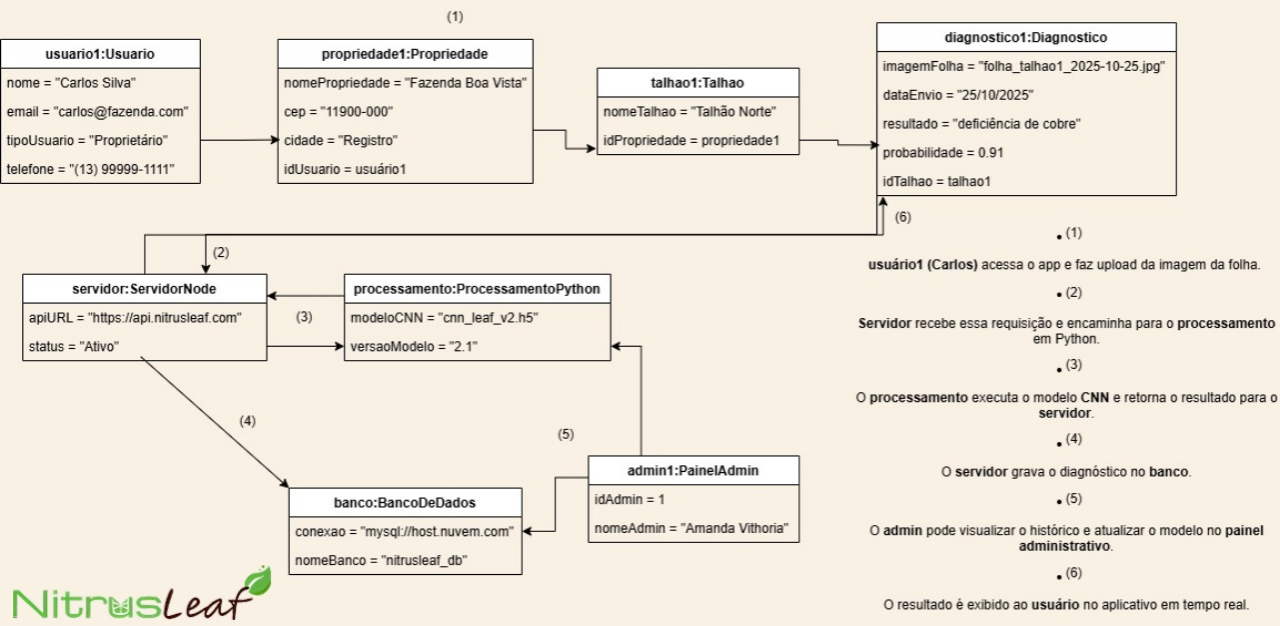
\includegraphics[width=0.8\textwidth]{Images/DiagramaDeObjetos.jpg}
\SourceOrNote{Equipe 21 - Vitalliz (2025)}
\end{figure}

O diagrama usa valores realistas (nomes, CEP, cidade, URLs) e encadeia o fluxo completo
do upload da folha pelo produtor até o diagnóstico gravado e exibido, com supervisão do admin
e versionamento do modelo.
\medskip